\begin{refsection}

\def\chaptertitle{Background: The ecology, biodiversity, structure and function of southern African woodlands}


\chapter[\chaptertitle]{\chaptertitle}
\chaptermark{Background}
\label{ch:background}

\section{Introduction}
\label{background:sec:intro}

Tropical savannas are expected to experience significant shifts in vegetation structure and biodiversity in the coming century, due primarily to human induced climate change, land use change, and changes in atmospheric carbon concentration \citep{Ross2021, Scheiter2009, Moncrieff2016}. Yet we lack a detailed understanding of how biodiversity and vegetation structure vary over space, and how that affects ecosystem function (i.e. processes controlling fluxes of energy and matter through ecosystems), resulting in large uncertainty in earth system flux estimates across this biome \citep{Ahlstrom2015}. This thesis examines the role of tree species diversity as a driver of ecosystem function, with a focus on woody biomass and productivity as measures of ecosystem function, in southern African savannas. Biodiversity - Ecosystem Function (BEF) theory predicts positive effects of biodiversity on ecosystem function \citep{Tilman2014}, but it is unclear whether this effect should occur in disturbance-prone and environmentally stressful ecosystems \citep{Steudel2012, Baert2018}. This chapter provides background on the ecology and biodiversity of tropical savannas and more specifically southern African savannas, then summarises current literature on biodiversity-ecosystem function theory, to understand in greater depth the rationale for this thesis.

\section{The ecology of savannas}
\label{background:sec:savanna}

Savannas occupy \textapprox{}20\% of the global land surface \citep{Scholes1993}. They are the dominant land cover in the seasonal tropics, covering \textapprox{}40\% of the tropical land surface \citep{Scholes1997} (\autoref{background:savanna_map}). While debate continues around use of the term `savanna' \citep{Lehmann2011, Ratnam2011}, the generic definition used in this thesis characterises a savanna by the co-dominance of grasses and trees, with a near contiguous grass-dominated understorey, and a closed or discontinuous, but sparse, woody overstorey \citep{Scholes1997, Bond2008}. Within this broad definition, savannas are highly heterogeneous, across local to continental scales \citep{Bucini2007}, with wide variation in canopy cover \citep{Sankaran2005, Hirota2011}, the structure and floristic composition of the woody overstorey \citep{Fayolle2018, Solbrig1996}, and the structure and composition of the herbaceous understorey \citep{Siebert2019, Coller2018}.

Historically, tropical savannas were often mis-represented as severely degraded forests \citep{Veldman2016}. This view has roots in the early twentieth century idea of Clementsian succession and potential vegetation \citep{Clements1916, Pulsford2014}, which focussed on hierarchical physiognomic vegetation classifications with closed canopy forest at the apex, rather than horizontal floristic or functional classifications that are in greater use at present \citep{Aleman2020}. The misinterpretation was exacerbated by the vast majority of early studies of savanna ecosystems originating from regions which lacked savanna vegetation. The hangover of this outdated paradigm is still felt today, with tropical savannas receiving less conservation funding \citep{Watson2016}, experiencing the greatest rates of transformation to agriculture of any major biome \citep{Hoekstra2004, Parr2014}, and being the focus of misplaced reforestation projects \citep{Silveira2020, Kumar2020, Laestadius2011}. In recent years there has been a push to acknowledge the value of tropical savannas, both intrinsically as centres of biodiversity and endemism \citep{Kumar2020, Pennington2018}, and as providers of ecosystem services \citep{Ryan2016}. Savannas proliferated globally during the Pliocene (\textapprox{}3-8 Mya), as a result of climate change, C\textsubscript{4} grass proliferation, and an increase in the frequency and intensity of fire, with all three of these causes being inter-linked \citep{Cerling1997, Beerling2006, Osborne2007, Edwards2010}. Rather than being viewed as derived landscapes that may be restored to a more forest-like environment, savannas should be considered a unique biome in their own right, with particular vegetation formations \citep{Torello2013}, a distinct evolutionary history \citep{Veldman2015}, and unique responses to global environmental change \citep{Sankaran2019}.

\begin{figure}[tb]
\centering
	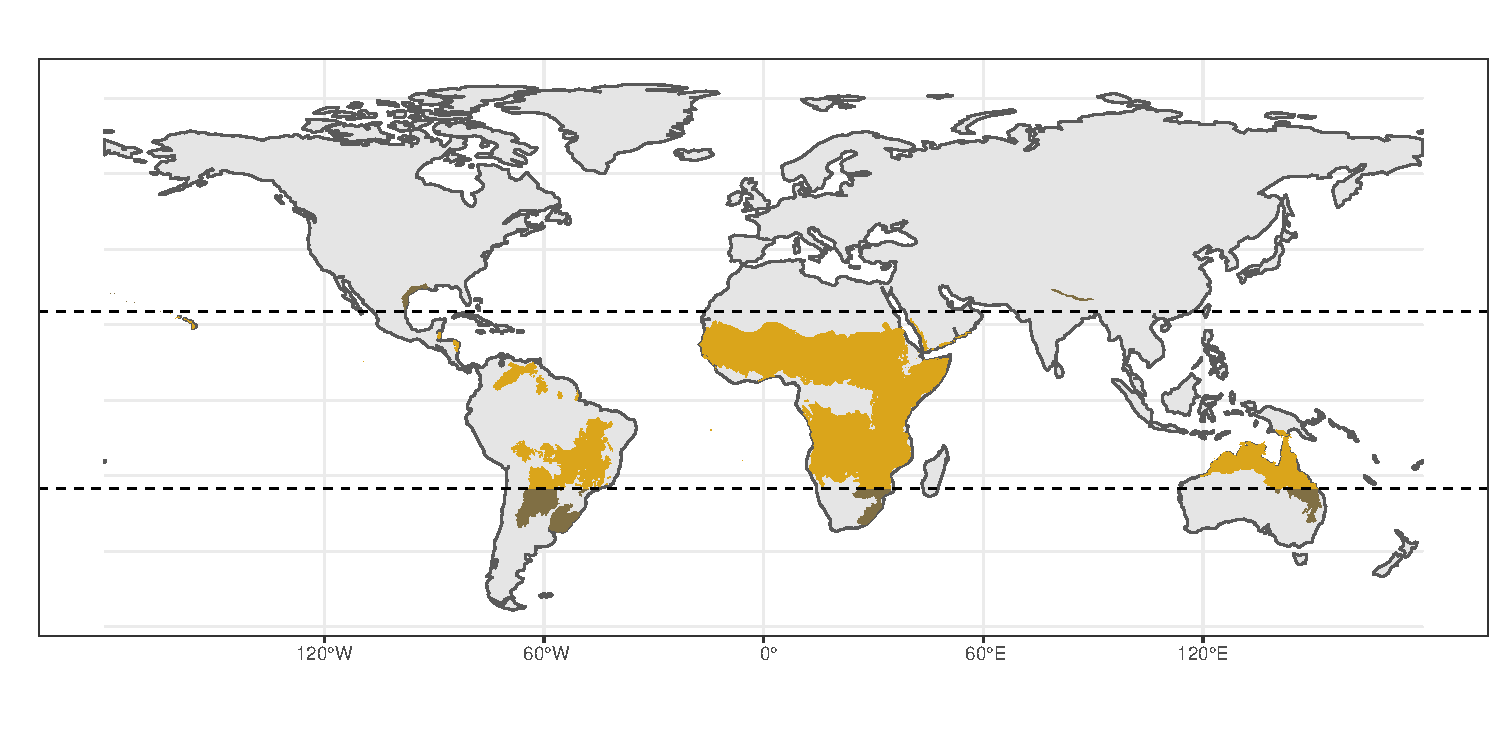
\includegraphics[width=\textwidth]{img/savanna_map}
	\caption[Map of global savanna distribution]{The global distribution of tropical savannas and grasslands (yellow), re-classified from the Terrestrial Ecoregions of the World \citep{Dinerstein2017}. Dashed lines mark the latitudinal extent of the tropics from N23.5\textdegree{} to S23.5\textdegree{}. Brown areas denote extra-tropical vegetation resembling tropical savannas.}
	\label{background:savanna_map}
\end{figure}

\subsection{Determinants of savanna vegetation}
\label{background:ssec:determ}

Savanna vegetation may occur as a result of multiple non-exclusive and interacting factors. One of the key questions in savanna ecology concerns identifying the factors driving variation in tree cover and woody biomass, and assessing their relative importance in different contexts, thus determining the global distribution of savannas \citep{Higgins2000, Archibald2019}. Controls on tree cover can be split broadly into `disturbance-based' (e.g. fire, herbivory) or `resource-based' (e.g. precipitation, soil fertility)  \citep{Bond2008, Staver2015}. Both resource-based and disturbance-based controls on tree cover act simultaneously to varying extents in most savannas, though it is possible to classify savannas into two principal biomes based on their dominant control on tree cover, through their effects on species composition and woodland structure \citep{Huntley1982, Torello2013}. 

Tropical savannas occur in areas of high rainfall seasonality \citep{Lehmann2011}. At the continental scale, available moisture is the most significant determinant of savanna tree cover \citep{Sankaran2005}, setting the upper boundary of tree cover by physiological limitation of tree growth. In wetter mesic savannas, competition between grasses and adult trees is low, but in arid savannas, grasses may `poach' water from trees by intercepting it closer to the soil surface \citep{Scheiter2007}. While water availability may be the dominant resource-based determinant of savanna vegetation, edaphic properties also affect tree cover across savannas. Tropical savannas are often associated with dystrophic soils, especially in higher rainfall areas, where available nutrients are leached from the soil \citep{February2013}. Furthermore soil texture also interacts with rainfall to allow greater woody biomass and less grassy biomass where the soil drains more readily \citep{Staver2011}. 

While resource availability, particularly moisture sets the upper bound for tree cover, many savannas exist in areas that are climatically suitable for closed canopy forest \citep{Sankaran2005, Lehmann2011, Staver2011, Murphy2012}. Even at local spatial scales, there exists large heterogeneity in woody canopy cover \citep{Dantas2015}. Above \textapprox{}650 mm yr\textsuperscript{-1}, woody cover in savannas appears to show no dependence on MAP \citep{Sankaran2008, Sankaran2005, Good2011}, suggesting that other factors such as soil and disturbance become more dominant above this precipitation threshold  \citep{Staver2011} (\autoref{background:map_cover_plain}). 

The key premise of the ``Alternative Stable States'' phenomenon is that contrasting ecosystem states may occur under similar environmental conditions, due to strong stabilising positive feedbacks on vegetation structure \citep{Staver2011}. Grass is the main fuel source for fires in mesic savannas. C\textsubscript{4} grasses, which dominate many mesic and arid savannas, particularly in southern Africa \citep{Still2003}, are particularly flammable, but require more light than C\textsubscript{3} grasses, meaning they are highly sensitive to variation in tree canopy cover \citep{CharlesDominique2018}. In areas with low grassy biomass, fire frequency and intensity are expected to be lower due to a lack of fuel. Simultaneously, juvenile trees are highly sensitive to fire in the grassy understorey layer due to their low stature, meaning that fire increases tree mortality, or `top-kill' of these individuals which must then resprout, keeping individuals small and creating a demographic bottleneck where only a few individuals grow to adults \citep{Bond1995, Ryan2011}. A positive feedback loop therefore occurs whereby disturbance by fire reduces canopy cover, allowing more frequent and intense fires, further reducing canopy cover as tree growth is suppressed. Alternatively, under reduced fire, trees can escape the `fire trap' in the understorey and grow to canopy trees \citep{Wakeling2011}, which rarely burn due to adaptive traits such as insulating bark and elevated crowns, increasing canopy cover, causing competitive exclusion of grasses \citep{Moustakas2013}, which further reduces disturbance by fire (\autoref{background:saf_theory}). 

\citet{Hirota2011}, using remotely sensed measures of tree cover across tropical Africa, South America and Australia, demonstrated a distinctly bi-modal distribution of tree cover within areas of intermediate rainfall (\textapprox{}650-1500 mm yr\textsuperscript{-1}). \citet{Staver2011} showed that fire was the main source of this bi-modality, and furthermore, \citet{Staver2017} showed that change in fire return interval, whether the result of management or environmental change, can result in transitions to an alternative stable state. Specifically, that longer fire return intervals result in a shift toward a more forest-like ecosystem with greater canopy closure, fewer small trees, and a greater number of large canopy trees.

\begin{figure}[tb]
\centering
	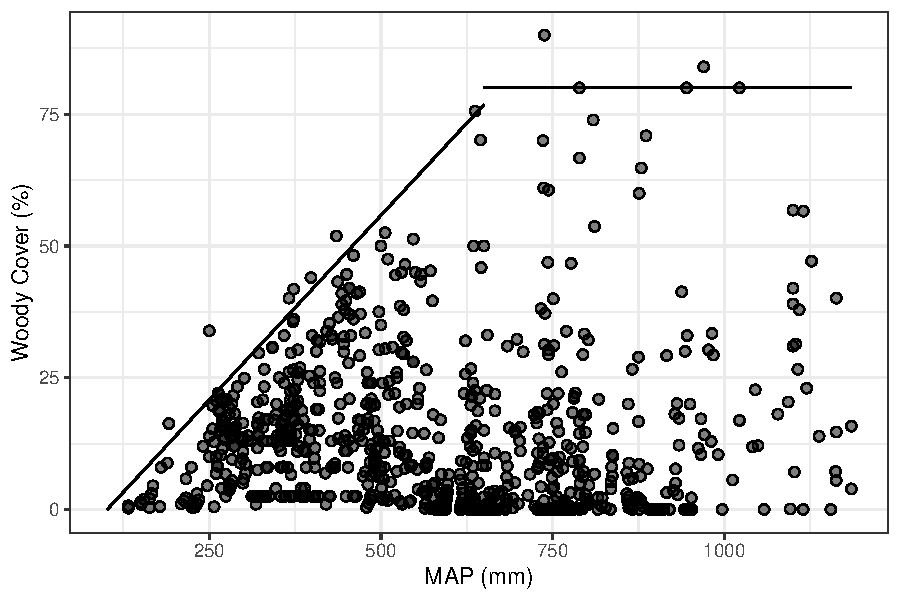
\includegraphics[width=\textwidth]{img/map_cover_plain}
	\caption[Precipitation vs. tree cover in southern Africa]{The relationship between rainfall (Mean Annual Precipitation) and proportional tree cover, across 854 savanna sites in Africa, adapted from \citet{Sankaran2005}. The line of best fit uses a broken-stick 99th quantile piece-wise linear regression to identify the breakpoint at which rainfall no longer sets the upper limit for tree cover. Above the breakpoint (650 $\pm$ 134 mm MAP) other processes such as disturbance by fire and local edaphic limitations are thought to determine tree cover.}
	\label{background:map_cover_plain}
\end{figure}

\begin{figure}[tb]
\centering
	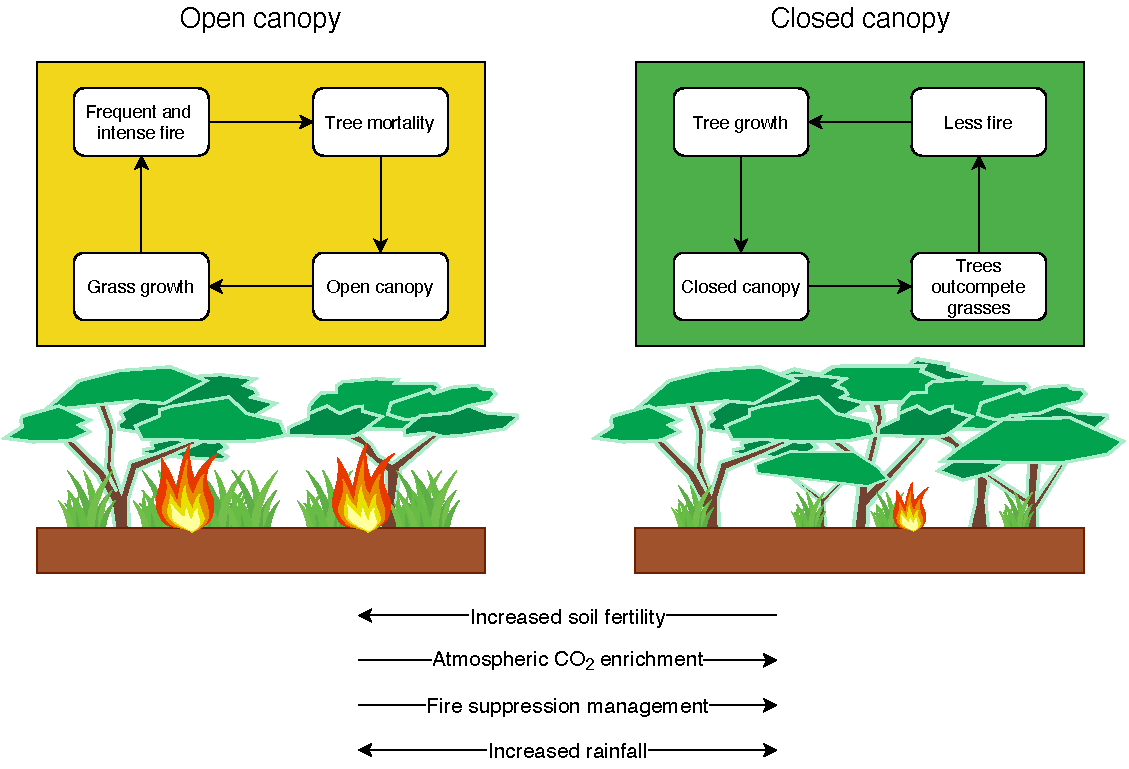
\includegraphics[width=\textwidth]{img/saf_theory}
	\caption[Schematic diagram of savanna positive feedback mechanisms]{The positive feedback mechanisms which determine the alternative stable states of mesic tropical savannas. Left: increased fire increases tree mortality, which decreases canopy cover, increasing available light for grass growth, leading to more fire and a further reduction in canopy cover. Right: decreased fire decreases tree mortality, which increases canopy cover, reducing available light to the grassy understorey, causing a reduction in grass fuel load, fewer fires and a further increase in canopy cover. Bottom: stabilising feedback loops can be disrupted given a large enough perturbation, causing a switch to another stable state. Some of these perturbations have different outcomes depending on the principal limitation of woody cover. In arid savannas, increased rainfall leads to an increase in woody cover, as more water percolates to deeper tree tap roots, while in a mesic savanna where water is not limiting, increased rainfall may lead to an increase in grass growth and therefore an increase in fire, which reduces woody cover.}
	\label{background:saf_theory}
\end{figure}

The factors described above which determine savanna vegetation structure are highly interactive. Moisture availability interacts with fire disturbance, leading, seemingly paradoxically, to a situation where increased resource availability may lead to lower woody biomass above a given threshold resource availability, due to increased grass growth and more intense and frequent fires \citep{Xu2015}. Soil fertility also plays an interactive role with fire, increasing grass recovery rate between fires, which may lead to more frequent fires, increased tree mortality and lower woody biomass \citep{Kellman1984}. Interactions between environment, disturbance and tree cover, with clear thresholds of resource availability and tipping points of disturbance regime, result in a highly complex model of savanna ecosystem processes. 

\subsection{Adaptations of savanna trees}
\label{background:ssec:adapt}

The model of ecosystem processes in savanna ecosystems described above, the result of interactions among water availability, soil fertility, and disturbance, only becomes more complex when the biotic component and its biogeographic variation is considered. Savanna trees are subject to a multitude of environmental pressures. To overcome these pressures, savanna trees have developed adaptations and employ various life history strategies, leading to high functional diversity within and among savanna ecosystems \citep{Solbrig1996}, despite their low tree species richness compared to tropical rainforests, for example. This functional diversity allows niche separation among species and potentially greater ecosystem function in higher diversity ecosystems, particularly by conferring greater resilience of function to environmental extremes such as drought \citep{Diaz2001}. This section describes some of the key adaptations of savanna trees and their effect on ecosystem processes.

Seasonal fires are a key determinant of savanna structure in mesic savannas (>650 mm MAP) \citep{Sankaran2005}. Many savanna tree species produce thick corky bark which protects the sapwood from high temperatures during fire \citep{Hoffmann2012, Lawes2011, Dantas2013}. Additionally, many savanna trees produce large below-ground root structures built to store carbohydrate, and access deep groundwater reserves, allowing individuals to re-sprout following fire \citep{Wigley2019}. There is evidence of adaptation in juveniles of some species that allows them to resprout in the same year following fire, giving them a head-start over competitors which adhere to a more rigid bud production cycle \citep{Wiegand2006}. Natural coppicing of adult savanna trees is common. If one growing tip is damaged due to fire, other stems on the same individual can continue growing, avoiding mortality. Savanna trees also sometimes have insulated buds to prevent fire reaching the sensitive growing tip \citep{CharlesDominique2015}.

Previously, root niche separation between grasses and trees was thought to be the main method by which trees and grasses coexist in savannas \citep{Walter1971}. Trees were observed to have deep tap roots while grasses have a greater density of fine near-surface roots \citep{Timberlake1993}. In arid savannas, root niche separation is an important mechanism allowing tree-grass coexistence, with consequences for the timing of seasonal growth in relation to seasonal rainfall intensity. In mesic savannas however, this effect is largely absent, except under specific edaphic conditions that increase soil drainage \citep{Case2020, Ketter2018, Sankaran2004, Higgins2000}. Recent work has shown that many savanna trees in mesic savannas produce two types of roots, the first are deep tap roots which are used primarily for water uptake and for storing carbohydrates as ligno-tubers to facilitate pre-rain green-up and resprouting following fire. The second are a mesh of finer roots which occur near to the surface and compete directly with grasses. These roots are used primarily for nutrient uptake, as most savanna soils have a distinct vertical nutrient profile \citep{Tomlinson2012, February2013}. In southern Africa particularly, many mesic savanna soils are denuded of phosphorus \citep{Campbell1996}. Thus, many dominant mesic savanna trees in the Fabaceae family, subfamily Detarioideae have mutualistic arbuscular mycorrhizal associations which improve phosphorus uptake \citep{Gomes2021}. Similarly, in drier savannas, many dominant non-Detarioideae Fabaceae species, including \textit{Acacia} spp., \textit{Dalbergia} spp., \textit{Dichrostachys} spp., etc, produce root nodules to host \textit{Rhizobia} capable of fixing atmospheric nitrogen \citep{Hogberg1986}. 

Seasonal fire routinely removes much of the grass layer in savannas, meaning that this is an ideal time for tree seedlings to germinate, as the lack of grass fuel means another fire is unlikely for some time, and the lack of grass cover means less competition for the growing seedling. Many tree species have adapted to having fire-activated seed dispersal \citep{Veldman2015}, with large seeds for long seed residence times, and rapid growth of newly emerged seedlings \citep{Daibes2019}, so that the seedlings can grow enough to escape the ``fire-trap'' before the grass fuel load has increased sufficiently to allow another fire. \citet{Wakeling2015} found that in densely grassy areas, a lack of gaps may prevent the germination of tree seeds, with long seed residence times allowing trees to take advantage of stochastic fire events that open up gaps for rooting. As an alternative to producing seed, many savanna trees reproduce predominantly via clonal growth. Clonal suckers remain connected to the natal tree, allowing rapid growth, as they benefit from the resources of the established carbohydrate-storing root structures \citep{Bond2003}.

Tropical savannas experience highly seasonal patterns of rainfall. Many savanna trees are deciduous, losing their leaves during the dry season to limit transpiration and conserve water \citep{Dahlin2016}. The phenomenon of `pre-rain green-up' has been observed widely across tropical savanna trees \citep{Archibald2007, Borchert1994, Williams1997, Ryan2017}, whereby trees produce foliage material in advance of the rainy season. Multiple mechanisms have been suggested to explain pre-rain green-up as an adaptive trait, such as: to optimize photosynthesis during the wet season \citep{Archibald2007}, to avoid herbivory \citep{Aide1988}, and to maximise the length of the growing season \citep{Scholes1993}. 

\section{Savannas and the global carbon cycle}
\label{background:ssec:carbon}

Tropical savannas contribute \textapprox{}30\% of global terrestrial Net Primary Productivity (NPP), i.e. atmospheric carbon fixed into biomass \citep{Grace2006}. Due to their large spatial extent, even a small percentage change in woody cover in savannas is expected to have large effects on the global carbon sink \citep{Williams2005}. Globally, savanna ecosystems are being degraded and lost to agricultural expansion, mining, and urban growth \citep{Parr2014}. \citet{Ross2021} predict biomass loss over most tropical savannas over the coming century, mostly due to land use change. Similarly, \citet{Aleman2016} concluded that land use change in sub-Saharan African savannas will have a greater negative effect on tree cover than changes in annual rainfall and rainfall seasonality. By 2100, the human population of sub-Saharan Africa is expected to double, increasing pressure on savanna ecosystems further \citep{Pison2017}. Despite this, tropical savannas are reportedly the fastest increasing component of the terrestrial carbon sink \citep{Sitch2015}, though they also represent the largest source of uncertainty in the terrestrial carbon cycle \citep{Ahlstrom2015}.

By 2050, it is expected that atmospheric CO\textsubscript{2} will have risen high enough that C\textsubscript{4} grasses no longer have a growth advantage over C\textsubscript{3} plants \citep{Bond2012}. An increase in atmospheric CO\textsubscript{2} is expected to lead to faster tree growth rates, allowing saplings to more quickly escape the ``fire-trap'', resulting in lower mortality, and a shift towards a closed canopy forest-like environment. Additionally, in arid savannas, the negative effect of CO\textsubscript{2} enrichment on grass transpiration rates \citep{Murphy2012} is expected to lead to less vigorous root growth and therefore more percolation of water to the deeper tree roots, increasing tree growth. Various studies, across the country of South Africa \citep{Stevens2016b}, the neotropics \citep{Rosan2019}, and globally \citep{Stevens2016}, have reported woody encroachment of trees into previously grassland or shrubland areas, increasing carbon uptake and storage in these systems. These studies cite atmospheric CO\textsubscript{2} increase as the main driver of this phenomenon. Due to the complex nature of the determinants of savanna tree cover however, it is still unclear whether the positive growth effects of CO\textsubscript{2} enrichment will occur to the same extent in different savanna ecosystems. Most global carbon cycling models currently use broad plant functional types to describe variation in function among biomes. It is common for all mesic savannas within southern Africa to be assigned to the same plant functional type, for example \citep{Atkin2015, Whitley2017}, yet we know there are many functionally distinct vegetation types in this region \citep{Campbell1996}, each likely to response to concomitant changes in environmental factors in different ways. 

\citet{Lewis2009} suggested that although existing woodlands are thickening, this does not necessarily extend to encroachment into previously unforested areas, due to the strong stabilising influence of fire. \citet{Pelletier2018} concluded that while more arid savannas will likely experience woody encroachment due primarily to the effects of CO\textsubscript{2} enrichment on transpiration and tree-grass water relations, there is no evidence that the same will happen in non-water limited savannas such as the miombo woodlands of southern Africa. Similarly, \citep{Reich2014} demonstrated that earth system models may be overly sensitive to the effects of CO\textsubscript{2} enrichment, and that the models suffer from a lack of mechanistic understanding of the effect of resource availability on disturbance. \citet{Korner2017} suggested that CO\textsubscript{2} enrichment may serve only to increase biomass turnover through increased growth offset by fire, with 44\% of all carbon emissions in savanna coming from fire \citep{Werf2010}, and 62\% of fire carbon emissions coming from savanna \citep{Werf2017}, offsetting the extra carbon sequestered.

Tropical savannas remain the largest source of uncertainty in models of the terrestrial carbon cycle \citep{Ahlstrom2015}. Environmental and land use change is expected to cause drastic changes to the functioning of savanna ecosystems in the coming century. Clearly, there is much work needed to better understand the mechanisms which determine the role of tropical savannas in the global carbon cycle. Carbon cycling models must consider biogeographic variation and the effect of functional differences among vegetation types on ecosystem functioning. In this thesis, I will explore the role of tree species biodiversity as a mediator of ecosystem functions related to carbon cycling, namely productivity and biomass storage. In doing so, I hope to provide a basis for incorporating information on biodiversity into carbon cycle models, to reduce their uncertainty in predicting the terrestrial carbon cycle.

\section{Southern African woodlands}
\label{background:sec:southern_african}

This thesis uses the mesic savannas of southern Africa as the main study location within which to explore the effects of biodiversity on ecosystem function. These savannas occur in a latitudinal band south of the Congo basin rainforest, and north of the arid savannas of the country of South Africa (\autoref{background:saf_map}), covering \textapprox{}2.7 million km\textsuperscript{2} \citep{Arino2010}. Hereafter they are referred to as southern African woodlands.

Tree cover in southern African woodlands is not primarily limited by precipitation, and instead are structured mainly by disturbance from fire and herbivory, leading to a highly heterogeneous patchy woodland habitat \citep{Archibald2019}. Fire return interval varies locally, dependent on climate and existing vegetation which determines grass fuel load \citep{Archibald2010}. Unlike fires in North American pine savannas, for example, fires in southern African woodlands rarely track up into the tree canopy, and instead burn quickly in the grass layer, causing tree mortality among juvenile trees but only occasionally in larger trees \citep{}. 

Large herbivores play an important role in determining the vegetation structure of southern African woodlands. Compared to climatically similar savannas in the neotropics or southeast Asia, large herbivores are common in savannas throughout southern Africa \citep{Asner2009}. It has been suggested that large herbivores may cause disturbance in a manner similar to fires, reducing woody biomass by increasing mortality of juvenile saplings \citep{Bond2005}, though the effects of herbivory are often much more localised than fire, and the spatial distribution of herbivory cannot be predicted with the same detail \citep{Hempson2015}. While the dominant pressure determining the coexistence of grass and trees in savannas globally is moisture availability, within southern African woodlands where rainfall is rarely a limiting factor, competition for light is more important \citep{Vadigi2013}. Depending on the disturbance regime, southern African woodlands occasionally form dense closed canopies, while C\textsubscript{4} grasses are highly sensitive to shade. Feedbacks between tree cover and grass growth determine the fire regime and lead to highly heterogeneous woodland structure.

Southern African woodlands support a growing human population, with >150 million people benefitting from ecosystem services provided \citep{Ryan2016, Wunder2014}. Vast areas of woodland in southern Africa are used for grazing cattle which requires relatively open woodland \citep{Njana2013}, while other areas are used for charcoal production, bushmeat hunting, fruit, vegetable and mushroom foraging, and timber production \citep{Ryan2016}. Wood extraction by humans is increasing in southern Africa \citep{Hansen2013}, with more than 90\% of harvested wood used for energy production, mostly as charcoal in a domestic setting \citep{May-Tobin2011}. Other important ecosystem services provided by these woodlands to the human population include regulation of water availability throughout the dry season \citep{Wilk2010, Hecky2003} and the provision of medicinal plants \citep{Ryan2016, Augustino2011}. Simultaneously, southern African woodlands are inhabited by a high number of charismatic endemic species \citep{Burgess2004} and are increasingly a destination for international tourists \citep{Vergles2015, Shackleton2007}. These attributes together make southern African woodlands a hugely important natural asset, both locally and globally.

Southern African mesic savannas can be divided roughly into three main vegetation types. Miombo woodlands dominate southern Africa, and are the largest savanna vegetation type in the world \citep{Ryan2011}. They are dominated by species from the Fabaceae family, subfamily Detarioideae, from the genera: \textit{Brachystegia}, \textit{Julbernardia}, and \textit{Isoberlinia}. The namesake `miombo' comes from the local name for the genus \textit{Brachystegia} in various Bantu languages. These woodlands frequently have tall continuous but sparse tree canopies, only occasionally closing to the point of excluding grasses. They are mistakenly classified as forest by some data-driven forest cover maps \citep{Hansen2013}, but the co-dominance of grasses and trees means that they are true savannas under the definition used in this thesis. Rainfall in miombo woodlands varies between 540-1700 mm yr\textsuperscript{-1}, with a highly seasonal pattern of precipitation. Many miombo tree species are deciduous, losing their leaves in the dry season to conserve water and limit chances of damage by embolism \citep{}. Miombo woodlands are diverse, with >8500 vascular plant species, of which >300 are tree species, many of which are endemic to the region \citep{Frost1996}.

Mopane woodlands form thin bands in the south of Zambia, Zimbabwe, central and southern Mozambique, and also across the border region of Angola and Namibia (\autoref{background:saf_map}). They are characterised by the dominance of a single tree species, \textit{Colophospermum mopane}, and generally occur in areas of lower rainfall than miombo woodlands \citep{Palgrave2003}. Reduced rainfall means that mopane soils are generally more fertile than the surrounding miombo woodlands \citep{Makhado2014}. Mopane woodlands are host to the largest diversity of large mammals in southern Africa, including populations of charismatic and highly threatened species such as the black rhinoceros (\textit{Diceros bicornis}) and giraffe (\textit{Giraffa camelopardalis}) \citep{Mittermeier2003}. While much of the mopane woodlands exists as short-stature shrubby vegetation, larger `cathedral mopane' exists in some areas, forming a near closed canopy \citep{Makhado2014}.

Baikiaea woodlands occur on sandy soils, in a wide belt along the Angolan-Namibian border to Zimbabwe. They are dominated by \textit{Baikiaea plurijuga}, which grow to large trees at low densities, with a long grass and shrub understorey that burns regularly \citep{Werger1978}. Like \textit{C. mopane}, \textit{B. plurijuga} is also in the Detarioideae subfamily. Baikiaea woodlands are generally less suitable for agriculture than miombo woodlands, with highly sandy soil and low rainfall, though logging pressures have removed many of the largest and oldest trees in some regions \citep{}. Like mopane woodlands, Baikiaea woodlands provide habitat for many large herbivores \citep{}.

Although this thesis focusses primarily on the mesic savanna types described above, other savannas not dominated by Detarioideae species also exist in southern Africa. Combretaceae woodlands are dominated by trees from the \textit{Combretum} and \textit{Terminalia}, both arbuscular mycorrhizal genera. Combretaceae woodlands are found in drier conditions than miombo woodlands, but still mainly on dystrophic soils. They differ from miombo woodlands in their woodland structure, lacking large canopy tree species \citep{}. Often, Combretaceae woodland patches can be found among miombo woodland patches, in areas where soil drainage or intense historic disturbance has precluded the growth of dominant miombo species \citep{}. Finally, Mimosoideae woodlands occur in drier eutrophic areas, often with higher levels of herbivory from large mammals than other woodlands in the region. Mimosoideae genera such as \textit{Acacia} often display `cagey' and thorny canopy architecture to protect from browsing mammals \citep{Maurin2014}. Mimosoid woodlands in southern Africa occur mainly in South Africa, Kenya and Tanzania \citep{}. Unlike the other vegetation types mentioned above, the tree cover in Mimosoid woodlands is more generally limited by precipitation \citep{}.

\begin{figure}[tb]
\centering
	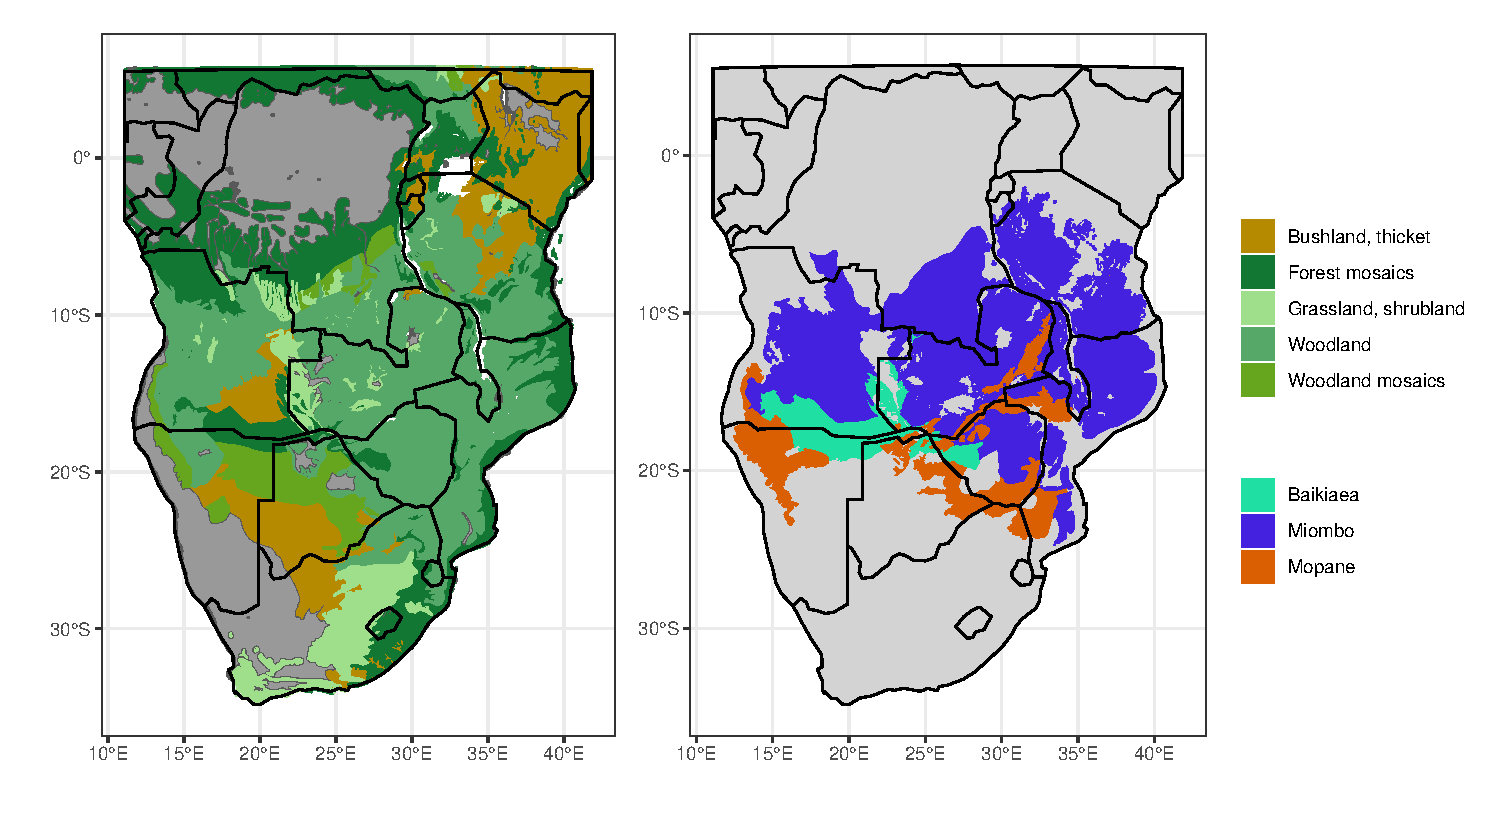
\includegraphics[width=\textwidth]{img/saf_map_both}
	\caption[Map of savanna vegetation types in Southern Africa]{The distribution of key savanna vegetation types within southern Africa. Left: physiognomic classification adapted from \citet{White1983}. Right: floristic classification of selected savanna-woodlands adapted from \citet{Dinerstein2017}, Terrestrial Ecoregions of the World.}
	\label{background:saf_map}
\end{figure}

\section{Biodiversity and ecosystem function theory}
\label{background:sec:befr_theory}

Since the development of the concept of niches \citep{Grinnell1904, MacArthur1967} and the coexistence of competing species \citep{Elton1927}, various research has touched on the potential link between species diversity, the efficiency of resource use, and therefore ecosystem function \citep{Hairston1960, Janzen1970, Grime1973, Whittaker1960}. In 1992, the Earth Summit in Rio de Janeiro discussed the growing concern that global patterns of biodiversity loss might negatively impact the functioning of ecosystems, and importantly damage the ecosystem services provided to humans. Later, researchers gathered in Bayreuth, Germany to discuss the role of biodiversity (B) on ecosystem function (EF), prompting the seminal work of \citet{Schulze1993}. Since then, a thriving field of research has emerged which aims to assess and explain the multiple and complex relationships between biodiversity and ecosystem function (\autoref{background:befr_graph}), with hundreds of studies exploring biodiversity effects in both experimental and natural systems \citep{Plas2019, Newbold2016, Tilman2014}. The 1992 Earth Summit defined a paradigm shift in ecological thinking. Previously, biodiversity had mainly been considered as a \textit{result} of environmental conditions and ecosystem function, while the research that came after redefined biodiversity as both a \textit{driver} and result of ecosystem function. BEF theory provides intuitive reasoning as to why increased biodiversity should lead to increased ecosystem function. 

BEF theory and supporting empirical evidence has informed global environmental policy by encouraging biodiversity conservation as a means of maintaining ecosystem functionality and its associated ecosystem services such as carbon storage, food provision, soil moisture retention etc. \citep{Balvanera2014, Naeem2012}. Increasingly, biodiversity conservation is encouraged as a method of indirectly maximising natural capital (perceived value of natural assets, \citealt{Kareiva2011}) by maximising ecosystem functionality \citep{Scherer-Lorenzen2014, Cardinale2012}. Many conservation policy makers are seeking win-win conservation strategies which will maximise both biodiversity and ecosystem service provision \citep{Howe2014, Adams2004}. Research into the role of biodiversity in maintaining ecosystem functionality has become more pertinent in the last 20 years in response to mounting evidence of startling global biodiversity losses \citep{McRae2017, Butchart2010, Vitousek1997}. There is trepidation however, that as ecosystems are transformed as a result of conservation meant to maximise ecosystem function, or rather a subset of ecosystem functions that are easily measured and have been identified as valuable, such as carbon sequestration \citep{Duffy2017}, other ecosystem functions and services may suffer and the ecosystem may lose unique characteristics \citep{Brockerhoff2017, Srivastava2005a}. 

This thesis aims to understand variation in ecosystem function across southern African woodlands through the lens of the ``Biodiversity - Ecosystem Function Relationship'' (BEFR). Ecosystem functions can be defined in broad terms as the rate processes which control the fluxes of energy and matter through an ecosystem \citep{Jax2005}. This includes basic processes of primary production such as gross primary productivity and atmospheric nitrogen fixation, but can be extended to indirect aggregate measures of function such as resilience of productivity to disturbance \citep{}. Additionally, ecosystem function can be further extended to ecosystem properties such as forest canopy complexity and trophic complexity, which in turn influence ecosystem processes. In this thesis, I focus on woody biomass, productivity, and tree cover as measures of ecosystem function, with the aim of improving our understanding of the vegetation and carbon dynamics of southern African woodlands.

\begin{figure}[p]
\centering
	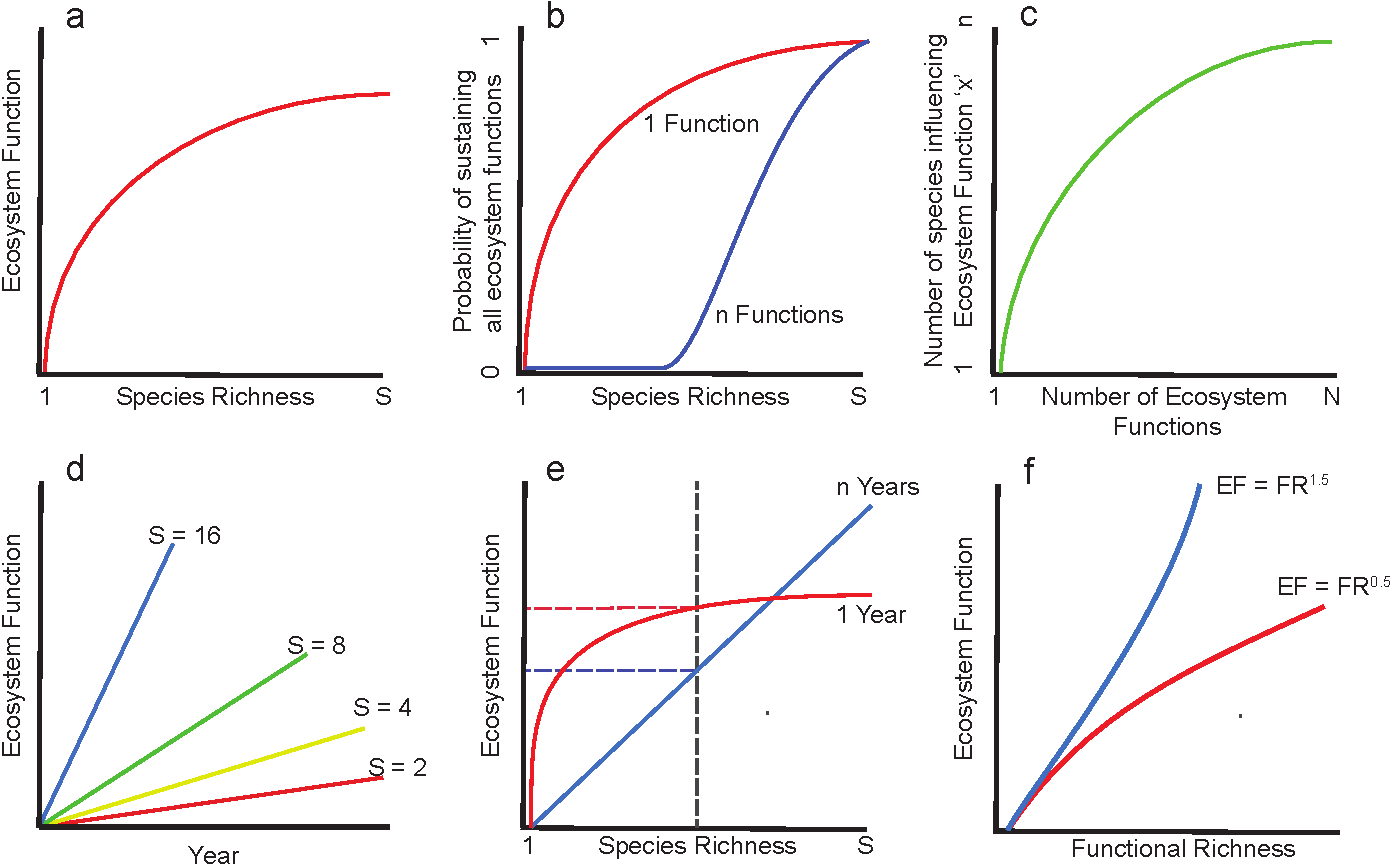
\includegraphics[width=\textwidth]{img/befr_graph}
	\caption[Inferences from previous Biodiversity-Ecosystem Function Research]{Schematic diagrams illustrating various inferences made on the Biodiversity - Ecosystem Function Relationship by previous studies. a) The classic BEF relationship found by many small scale experiments \citep{Cardinale2009}. b) As more functions are considered simultaneously the minimum species richness needed to maintain overall ecosystem functionality increases, also showing how the proportion of functionally redundant species increases as less functions are considered (i.e. the curve reaches asymptote at a lower species richness) \citep{Hector2007}. c) The saturating relationship of the number of ecosystem functions considered and the number of species influencing ecosystem multifunctionality \citep{Hector2007}. d) As studies progress through time the strength of the BEF relationship increases, the rate of increase in ecosystem function increases as species richness (S) grows \citep{Cardinale2007}. e) As studies progress through time the shape of the relationship becomes more linear, saturating at progressively higher species richness. Studies averaged over longer periods exhibit a greater loss in ecosystem function in response to an equivalent species richness reduction \citep{Reich2012}. f) When functional richness is used in place of species richness, the relationship reaches asymptote at a higher richness. Additionally the relationship becomes more concave as a power coefficient representing the strength and number of species interactions increases. FR\textsuperscript{>1} (interspecific competition > intraspecific competition (unstable)) results in a convex relationship, while FR\textsuperscript{<1} results in a concave relationship \citep{Mora2014}.} 
	\label{background:befr_graph}
\end{figure}

\subsection{Niche complementarity, selection effects, and facilitation}
\label{background:ssec:niche}

% Selection effects
There are various mechanisms underlying the observed effect of biodiversity on ecosystem function. Early experiments in artificial grasslands \citep{Tilman1994} and experimental microcosms \citep{Naeem1994}, which involved introducing or removing species from random assemblages concluded that \textit{selection effects} were the strongest drivers of the BEFR. Assuming random introduction or extinction of species, it is more likely that a diverse community will contain a species which contributes to a given ecosystem function \citep{Huston1997}. Of course, in natural systems, species introduction and removal is rarely random and may be confounded by a species' contribution to ecosystem function \citep{Smith2003}. Related to selection effects, which place emphasis on the presence of species which contribute to function, \citet{Grime1998} proposed the Mass-Ratio Hypothesis to explain biodiversity effects on ecosystem function. The Mass-Ratio Hypothesis suggests that it is not the breadth of niche space filled by a species assemblage that determines ecosystem function, but the ability of the most abundant species to optimise a chosen ecosystem function. Subsequent experimental studies have attempted to partition selection effects from other effects, or to remove selection effects entirely through experimental design, in an attempt to isolate other effects \citep{Loreau2001a}.

% Niche complementarity
The mechanism of niche complementarity has been the main focus of the majority of previous BEFR studies (\autoref{background:niche_all}) \citep{Wright2017}. The theory of niche complementarity follows intuitively from early evolutionary theory, that coexisting species must occupy different environmental niches, in order to prevent competitive exclusion of the weaker competitor \citep{Tobner2016, Levine2009, MacArthur1955, MacArthur1967}. Thus, the more species present in a given system, the more environmental niche space is filled, leading to more efficient and complete use of resources, a reduction in density dependent intra-specific competition and `higher' observed values for various ecosystem functions \citep{Isbell2013}. The mechanism of niche complementarity has been corroborated by many studies, but to varying extents depending on biome, whether the study was conducted in an experimental or natural system, the duration of study, and what measures of biodiversity and ecosystem function are used \citep{Wright2017, Cardinale2009, Cardinale2011}. Niche complementarity can also mediate functionality over time, as different species are able to optimise function at different times under under varying environmental conditions; this effect is known as the biodiversity insurance hypothesis \citep{Morin2014b, Bartomeus2013, Yachi1999a}. The insurance hypothesis also postulates that higher biodiversity at the landscape level will increase the rate at which ecosystems recover from stochastic local disturbances, by providing refugia populations in less perturbed areas \citep{Gonzalez2009}. 

% Facilitation
Facilitation effects increase the functional contribution of certain species in combination. For example, if grass species A is sensitive to high temperatures, tree species B may provide shade and thus reduce the temperature of the understorey, increasing the productivity of grass species A compared to if it was found in monoculture. Originally this specific example of facilitation was termed ``nurse plant syndrome'' \citep{Padilla2006}. This effect has been studied extensively in dryland ecosystems, where adult trees act as nurse plants for juveniles below, providing shade and reducing mortality. \citet{Callaway1997, Good2014, Weltzin1999} theorised a predictable relationship between environmental stress and the nature of interactions among plants, hypothesising that facilitation effects override competitive effects in highly stressful environments. More recently, \citet{Lortie2021} conducted a meta-analysis of facilitation effects in arid shrublands, concluding that while shrubs do provide facilitative effects, the net effect of species diversity on shrub biomass turned weakly negative under high diversity, due to competitive effects. Facilitation effects remain understudied in the BEFR literature. A history of research into partitioning niche complementarity from selection effects in biodiversity experiments has largely ignored the role of facilitation effects, presumably because they are not expected to drive large scale variation in the BEFR between systems, and because they are often context specific and difficult to test for their presence in natural systems \citep{Wright2017}. \citet{Wright2021} discusses how facilitation effects may have been mistakenly identified as niche complementarity as a result of the simplistic partitioning method used in previous studies.

\begin{figure}[p]
\centering
	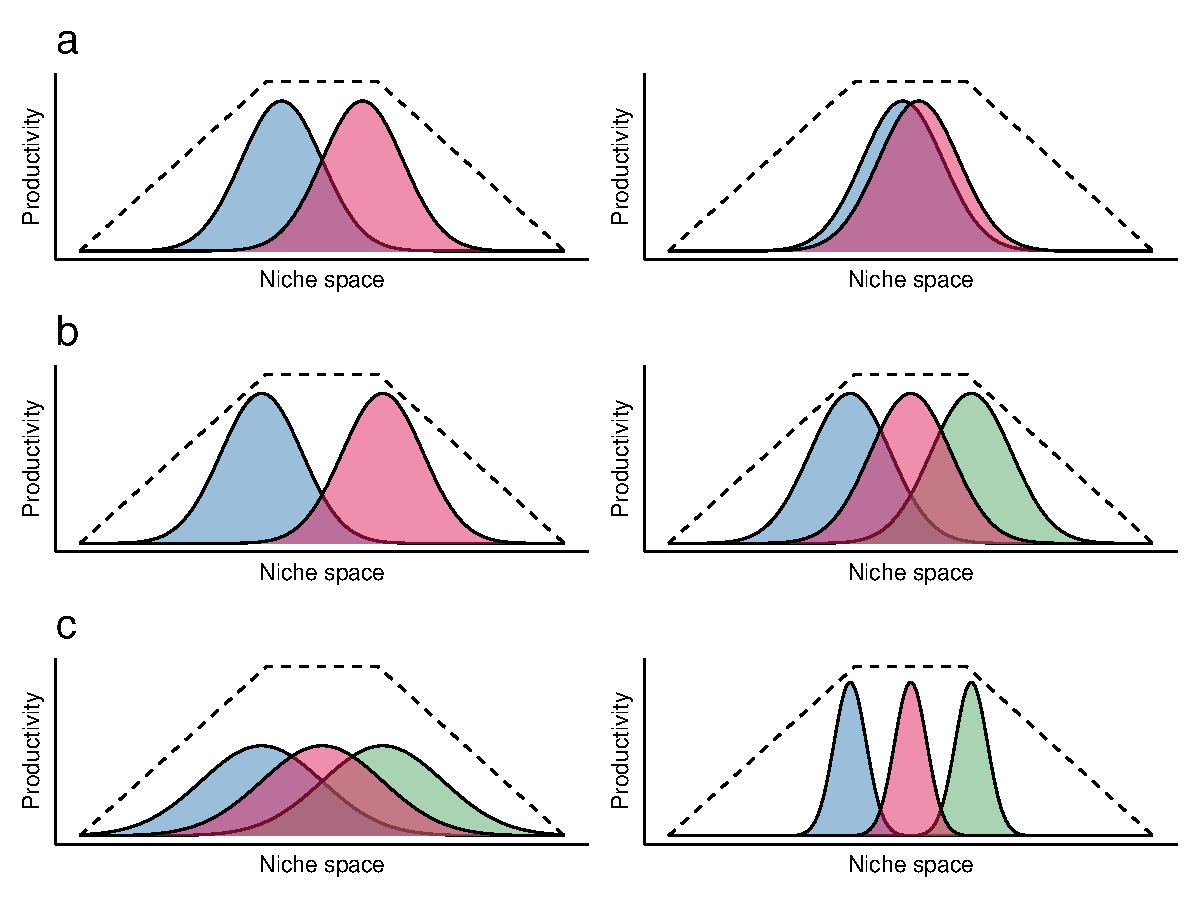
\includegraphics[width=\textwidth]{img/niche_all}
	\caption[Schematic diagrams demonstrating secondary controls on niche complementarity]{Schematic diagrams demonstrating niche occupation and secondary controls on the mechanism of niche complementarity. Each density plot shows a number of species, each represented by the species functional contribution (productivity) under different environmental conditions (niche space) within the larger environmental niche volume (dashed line). a) shows how the degree of overlap in functional niche of two species affects the total utilisation of the environmental niche volume (area under all species curves). When species are functionally distinct (left), more of the environmental niche volume is utilised. Removal of a species in this case would result in a large reduction in ecosystem productivity, while on the right, where functional redundancy is high, removal of a single species would have negligible effects. b) shows the effect of adding a functionally distinct species to an ecosystem. c) shows the effect of niche breadth on niche volume utilisation. On the left, three generalist species overlap in their functional niche. While each species has relatively incomplete utilisation of the environmental niche volume, this is offset as each species may occupy a wide range of environmental conditions. If the red species was removed, there would be only a marginal reduction in ecosystem productivity. On the right, three specialist species have a narrower niche breadth but a more complete utilisation of the environmental niche under ideal conditions. If a species was removed from this ecosystem, there would be a much greater reduction in ecosystem productivity.}
	\label{background:niche_all}
\end{figure}

\subsection{Global distribution of biodiversity-ecosystem function research}
\label{background:ssec:befr_global}

Among the hundreds of published studies of the biodiversity-ecosystem function relationship (BEFR), the majority are from experimental contexts, in small grassland patches or mesocosms. The number of studies in forested ecosystems is growing, but remains restricted predominantly to temperate forests in the global north \citep{Clarke2017}. In particular, there is a paucity of BEFR research in disturbance-prone wooded ecosystems, e.g. the mesic savannas which cover \textapprox{}20\% of the global land surface \citep{Scholes1993}. \citet{Liang2016} conducted a meta-analysis of estimates of the BEFR from 777,126 forest sample plots. They found that 99.87\% of these estimates followed a monotonic, positive BEFR curve, which saturated at high species richness. However, less than 600 of these plots were located in Africa, and none further south than Tanzania. 

\citet{Clarke2017} reviewed four BEFR meta-analyses \citep{Gamfeldt2015, Griffin2013a, Zhang2012, Cardinale2009} and identified only two studies conducted in Africa \citep{Foster1999, Burleigh1997}, compared with 69 in Europe and 82 in North America (\autoref{background:befr_map}). Both of these African studies are narrow in their scope and do not consider southern African woodland-savanna mosaics. \citet{Foster1999} studied the effect of dietary diversity on a single marine mollusc species in an experimental context. \citet{Burleigh1997} is an agroforestry study primarily investigating the suitability of two Fabaceae tree species as erosion mitigators. Neither of these studies provide an understanding of the BEFR that is relevant to understanding how entire savanna ecosystems respond to changes in biodiversity. In \citeauthor{Duffy2017}'s \citeyearpar{Duffy2017} meta-analysis, only three terrestrial field studies from southern Africa were used to compare the effects of biodiversity to those of environmental factors from a total of 167 field estimates of the BEFR. Given the unique community composition \citep{Lehmann2011}, environmental conditions \citep{Linder2003} and strong role of disturbance by fire and herbivory in structuring these savannas \citep{Staver2011}, it would be simplistic to generalise the BEFR found in other systems to this region.

\begin{figure}[tb]
\centering
	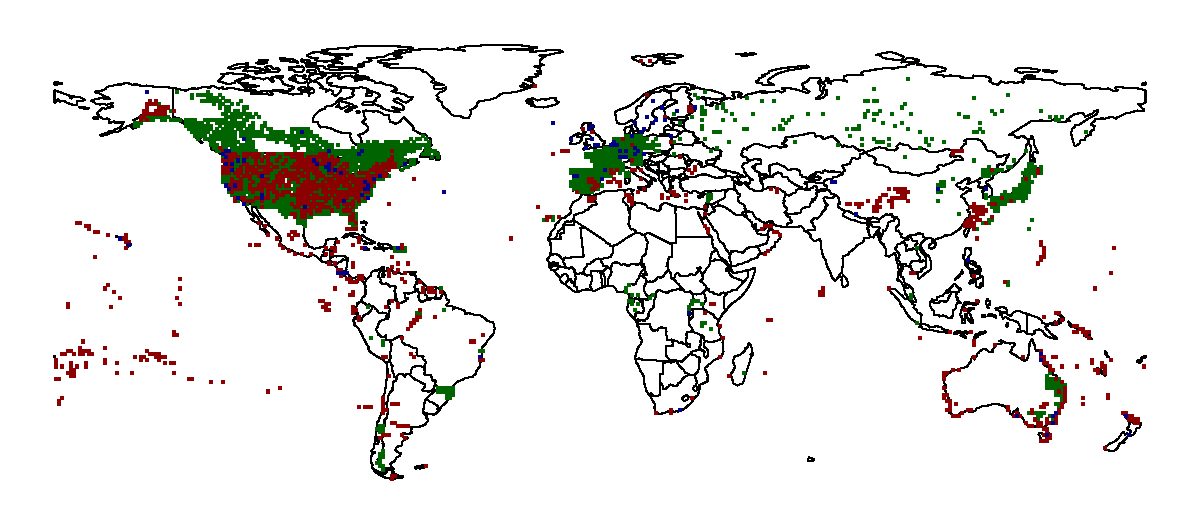
\includegraphics[width=\textwidth]{img/befr_map}
	\caption[Global distribution of Biodiversity-Ecosystem Function Relationship studies]{Location of studies of the biodiversity - ecosystem function relationship included in three meta-analyses of BEF research: blue \citet{Clarke2017}, green \citet{Liang2016}, red \citet{Duffy2017} - 67 field studies.}
	\label{background:befr_map}
\end{figure}

\subsection{Should we expect biodiversity effects on ecosystem function in southern African woodlands?}
\label{background:ssec:befr_africa}

Extensive research has linked tree biodiversity to ecosystem function in temperate and tropical forests \citep{Liang2016}, but only a small number of BEFR studies have taken place in tropical woodlands, and fewer still in southern African woodlands. The effects of disturbance and water availability in particular, which serve to reduce tree cover and biomass in southern African woodlands, might weaken or even invert the positive biodiversity-ecosystem function relationship found in other biomes \citep{Tilman2012a, Tilman2014, Hooper2012}.

In temperate and wet tropical closed canopy forests trees interact with each other due to their close proximity \citep{Coomes2007a, Purves2007}. Overlapping canopies and inter-weaving root networks produce competition for light, water and nutrients among individuals. Southern African woodlands however, exist along a wide gradient of tree cover. At the extreme low end of this gradient, trees may be too far apart for canopy competition to occur, and while the root networks of savanna trees are often extensive \citep{Belsky1994}, root competition may also be negligible among adult trees in the most sparsely wooded ecosystems. Though \citet{Dohn2017} demonstrated strong competitive interactions at neighbourhood scales of up to 5 m for most trees in an East African savanna. Low tree densities may result from a combination of resource-based processes such as low water availability and disturbance caused by fire, herbivory, or human land use practices such as selective logging \citep{Ryan2016}. \autoref{background:map_cover_plain} shows observed woody cover along a precipitation gradient in Africa, taken from \citet{Sankaran2005}. It shows that in the majority of plots, woody cover is below the physiological maximum set by precipitation, indicating that many other factors influence woody cover other than water availability. A lack of competition would weaken the effect of tree species diversity on ecosystem function, as multiple species can often fill overlapping niches in the absence of competition. In other words, the lack of competition allows the realised niche of a species to expand to approach the fundamental niche set by physiological limitations. Niche differentiation however, would still occur, only allowing certain species to establish and optimise productivity in certain micro-habitats, suggesting at least some effect of tree diversity on ecosystem function even in the most sparsely forested ecosystems. 

While disturbance and low resource availability may reduce the strength of biodiversity effects in southern African woodlands through its effect on competition, these same environmental pressures may increase the strength of the BEFR via facilitation effects. In European forests, \citet{Ratcliffe2017} found that the strength of the effect of tree species richness on many ecosystem functions increased as water availability decreased. They suggested that facilitation effects between species became stronger than competitive effects when resource availability was low, with strong facilitation effects being more likely at high species richness. Furthermore, \citet{Baert2018} reported that environmental stress shows a humped relationship with the strength of the BEFR, with the relationship being highest at intermediate levels of stress. They suggest an interplay between niche complementarity and selection effects at low environmental stress levels, which are often accompanied by greater levels of competition due to the lack of growth limitation, and higher facilitative effects at very high levels of environmental stress. \citet{Cardinale2002} found that in an experimental mesocosm of caddisfly larvae, increased disturbance in the form of random individual mortality led to increased effects of species richness on productivity. They attributed this effect to a decrease in dominance of competitively superior but low productivity taxa. Fire disturbance in forests has been linked to abundance dependent mortality among smaller stems \citep{Roques2001}. A species with more small stems is more likely to experience mortality during a fire. There may therefore be a link between disturbance regime and the strength of the species richness - ecosystem function relationship in fire prone woodland ecosystems. Unlike the caddisfly larvae in \citet{Cardinale2002} however, tree species differ in their resilience to fire driven mortality, owing to adaptations such as corky bark \citep{Solbrig1996}. The strength of the BEFR in a given system may therefore be a product of environmental conditions, disturbance regime, and species functional composition. These factors, which remain unmeasured in many studies of the BEFR in natural systems may explain some of the variation in the observed strength of the BEFR, and may be especially important in determining the BEFR in southern African woodlands. Conducting experiments across environmental gradients will improve understanding of how biodiversity effects interact with the environment to determine ecosystem functionality \citep{Turnbull2016, Tilman2014}. 

\subsection{Structural diversity, tree cover and ecosystem function}
\label{background:ssec:struc}

Biodiversity in BEFR studies is most often measured as the species richness of a focal trophic level or functional group (e.g. trees). However, more complex measures such as functional richness provide better insight into the tangible organism level processes which drive biodiversity effects \citep{Finegan2015, Scherer-Lorenzen2014, Petchey2006}. For example, increased tree species richness appears to cause an increase in the productivity of forest stands, but is this due to a greater likelihood of including a productive species (selection effects), canopy packing complementarity, root depth complementarity, facilitative shading effects, or more likely a combination of all the above? Investigating the mechanisms responsible for biodiversity effects provides better understanding of ecosystem processes, and allows for more generalisable predictions of the effects of species loss on ecosystem function.

Structural diversity, also referred to as structural complexity, i.e. variation in tree size and physiognomy, is one important measure of functional diversity in wooded ecosystems \citep{Ali2016, Ali2019, Pedro2017, Lecina-Diaz2018}. In disturbance-prone southern African woodlands, while some trees remain small, resprouting and coppicing after each fire to produce shrub-like understorey trees e.g. \textit{Baphia massaiensis}, others grow rapidly to escape the fire zone, producing large, spreading canopy trees, e.g. \textit{Julbernardia paniculata}. This variation in growth strategy among species that would otherwise compete for canopy space allows greater total canopy cover, foliage area, and presumably Gross Primary Productivity (GPP) in woodlands with greater tree species diversity. \citet{Seidel2013} and \citet{Danescu2016} both found that species richness increases tree canopy density and productivity in European temperate forest. Similarly, \citep{Neill2013} found that canopy structural complexity was related to ecosystem resilience and recover from disturbance. 

In addition to inter-specific variation in growth strategy as a driver of structural diversity, the spatial distribution and relative size of trees, i.e. stand structure, is also expected to affect canopy structural complexity \citep{}. Disturbance history and fine-scale environmental heterogeneity affect the vertical and horizontal distribution of tree canopies. Complex feedbacks may therefore be at play, where disturbance influences structural diversity and canopy structure, which in turn influences disturbance. It is unclear however, what the full effect of stand structure is on canopy cover in southern African woodlands, and how it compares to other drivers of canopy cover. Understanding the effects of species diversity and stand structure on canopy packing and tree cover will not only improve our understanding of the mechanisms underlying biodiversity effects on productivity, but also offers insight into the dynamics of woody encroachment, and why some woodland canopies close more readily to exclude grasses \citep{Staver2011}.

\section{Conclusions}
\label{background:sec:conclusion}

Tropical savannas are complex, and savanna vegetation arises as a result of many interacting factors, but are understudied and represent the largest uncertainty in models of the global carbon cycle. Assumptions about the behaviour of tropical savannas cannot be based on other tropical forested ecosystems, mainly due the pervasive effect of disturbance and resource scarcity on ecosystem function. Previous studies of tropical savannas have focussed predominantly on the role of abiotic environment and disturbance as drivers of ecosystem function, with biodiversity as a passive result of these factors. Biodiversity - Ecosystem Function research reframes the role of biodiversity as both a driver and result of ecosystem function, and provides an intuitive prediction that biodiversity increases ecosystem function. However, BEF research in natural forested ecosystems has shown that both positive and negative biodiversity effects may occur, depending on the function studied and the intensity of environmental stress. It is unclear how biodiversity of tree species in southern African woodlands may affect productivity, but there are multiple reasons why biodiversity effects might be weaker or possibly negative in this biome. This thesis aims to increase our understanding of tree biodiversity in southern African woodlands, the world's largest savanna, through the lens of the Biodiversity-Ecosystem Function Relationship.

\newpage{}
\begingroup
\setstretch{1.0}
\printbibliography[heading=subbibintoc]
\endgroup

\end{refsection}

